\documentclass[../main.tex]{subfiles}
\begin{document}
%%%%%%%%%%%%%%%%%%%%%%%%%%%%%%%%%%%%%%%%%%%%%%%%%%%%%%%%%%%%%%%%%%%%%%%%%%%
%%%%% Examples
%%%%%%%%%%%%%%%%%%%%%%%%%%%%%%%%%%%%%%%%%%%%%%%%%%%%%%%%%%%%%%%%%%%%%%%%%%%

In this chapter, we mainly discuss about the array based questions. We first categorize these problems into different type, and then each type can usually be solved and optimized with nearly the best efficiency. 

Given an array, a subsequence is composed of elements whose subscripts are increasing in the original array. A subarray is a subset of subsequence, which is contiguous subsequence. Subset contain any possible combinations of the original array. For example, for array [1, 2, 3, 4]:
\begin{lstlisting}[numbers=none]
Subsequence
[1, 3]
[1, 4]
[1, 2, 4]
Subarray
[1, 2]
[2, 3]
[2, 3, 4]
Subset includes different length of subset, either
length 0: []
length 1: [1], [2], [3], [4]
length 2: [1, 2], [1, 3], [1, 4], [2, 3], [2, 4], [3, 4]
\end{lstlisting}

Here array means one dimension list. For array problems, math will play an important role here. The rules are as follows:
\begin{itemize}
    \item Subarray: using dynamic programming based algorithm to make brute force $O(n^3)$ to $O(n)$. Two pointers for the increasing subarray. Prefix sum, or kadane's algorithm plus sometimes with the hashmap, or two pointers (three pointers) for the maximum subarray. 
    \item Subsequence: using dynamic programming based algorithm to make brute force $O(2^n)$ to $O(n^2)$, which corresponds to the seqence type of dynamic programming. 
    \item Duplicates: 217, 26, 27, 219, 287, 442;
    \item Intersections of Two Arrays: 
\end{itemize}

Before we get into solving each type of problems, we first introduce the algorithms we will needed in this Chapter, including two pointers (three pointers or sliding window), prefix sum, kadane's algorithm. Kadane's algorithm can be explained with sequence type of dynamic programming. 

    % Easy problems: Duplicates:  Intersection: 349. Intersection of Two Arrays; Consecutive: 485. Max Consecutive Ones
    % Maximum/Minimum subarray: 718, 53. Maximum Subarray, 325. Maximum Size Subarray Sum Equals k. 209. Minimum Size Subarray Sum Solutions: divide and conquer, special sum and hashtable, two pointers (sliding window) for minimum
    % Sum of K numbers of elements: Target, return either the index or the elements(might need to avoid repetition). (2/3/4 sums)
    % Partition a list into K equal part: DP
    
After this chapter, we need to learn the step to solve these problems:
\begin{enumerate}
    \item Analyze the problem and categorize it.  To know the naive solution's time complexity can help us identify it.
    \item If we can not find what type it is, let us see if we can \textit{convert}. If not, we can try to identify a simple version of this problem, and then upgrade the simple solution to the more complex one. 
    \item Solve the problem with the algorithms we taught in this chapter.
    \item Try to see if there is any more solutions. 
    

    % \textit{Note: If the problem is complex, trying to see the simple version, and then upgrade the simple version to a complex one. e.g. (487. Max Consecutive Ones II, 485. Max Consecutive Ones)}
    \item Check the special case. (Usually very important for this type of problems)
\end{enumerate}
% Including two pointers both from the start, or two pointers one is from the beginning and the other is from the end. Also, the sliding window, and the flexible sliding windows, also find the cycle algorithm. 
%%%%%%%%%%%%%%%%%%%%%%%%%%%%%%%%%%%%%%%%%%%%%%%%%%%%%%%%%%%%%%%%%%%%%%%%%%%
%%%%% Subarray
%%%%%%%%%%%%%%%%%%%%%%%%%%%%%%%%%%%%%%%%%%%%%%%%%%%%%%%%%%%%%%%%%%%%%%%%%%%
\section{Subarray }
\textit{Note: For subarray the most important feature is contiguous. Here, we definitely will not use sorting.} Given an array with size $n$, the total number of subarrays we have is $\sum_{i=1}^{i=n} i = n*(n+1)/2$, which makes the time complexity of naive solution that use two nested for/while loop $O(n^2)$ or $O(n^3)$. 

There are two types of problems related to subarry: \textbf{Range Query} and \textbf{optimization-based subarray}.  The Range query problems include querying the minimum/maximum or sum of all elements in a given range [i,j] in an array. Range Query has a more standard way to solve, either by searching or with the segment tree:
\paragraph{Range Query}
\begin{enumerate}
    \item 303. Range Sum Query - Immutable
    \item 307. Range Sum Query - Mutable
    \item 304. Range Sum Query 2D - Immutable
\end{enumerate}

\paragraph{Optimization-based subarray} 
Given a single array, we would normally be asked to return either the maximum/minimum value, the maximum/minimum length, or the number of subarrays that has sum/product that \textit{satisfy a certain condition}. The condition here decide the difficulty of these problems.

The questions can are classified into two categories:
\begin{enumerate}
    \item \textit{Absolute-conditioned Subarray} that $sum/product=K$ or 
    \item \textit{Vague-conditioned subarray} that has these symbols that is not equal.
\end{enumerate}

% \begin{enumerate}
%     \item Maximum/minimum subarray with Sum or Product or a pattern; we use \textbf{math and prefix\_sum} or sometimes together with hashmap method to tackle. Also, sliding window can be used.
%     \item Minimum Subarray with Sum or Product or a pattern; \textbf{sliding window} can be used to get the minimum length of subarray. 
%     \item Find subarray that is increasing or decreasing ; \textbf{Two pointers or sliding window} can be used. 
% \end{enumerate}
With the proposed algorithms, the time complexity of subarray problems can be decreased from the brute force $O(n^3)$ to $O(n)$. The brute force is universal: two nested for loops marked the start and end of the subarray to enumerate all the possible subarrays, and another $O(n)$ spent to compute the result needed (sum or product or check the pattern like increasing or decreasing). 

% Using prefix sum or kadane's algorithm or hashmap sometimes if we have problems to solve it, a panacea is the Sliding Window Algorithm either with two or three pointers. 

As we have discussed in the algorithm section, 
\begin{enumerate}
    \item \textbf{stack/queue/monotone stack} can be used to solve subarray problems that is related to its smaller/larger item to one item's left/right side
    \item \textbf{sliding window} can be used to find subarray that either the sum or product inside of the sliding window is ordered (either monotone increasing/decreasing). This normally requires that the array are all positive or all negative. We can use the sliding window to cover its all search space. Or else we cant use sliding window. 
    \item For all problems related with subarray sum/product, for both vague or absolute conditioned algorithm, we have a universal algorithm: save the prefix sum (sometimes together with index) in a sorted array, and use binary search to find all possible starting point of the window. 
    \item Prefix Sum or Kadane's algorithm can be used when we need to get the sum of the subarry. 
\end{enumerate}

\begin{enumerate}
    \item 53. Maximum Subarray (medium)
    \item 325. Maximum Size Subarray Sum Equals k
    \item 525. Contiguous Array
    \item 560. Subarray Sum Equals K
    \item 209. Minimum Size Subarray Sum (medium)
\end{enumerate}
Monotone stack and vague conditioned subarray
\begin{enumerate}
    \item 713. Subarray Product Less Than K (all positive)
    \item 862. Shortest Subarray with Sum at Least K (with negative)
    \item 907. Sum of Subarray Minimums (all positive, but minimum in all subarray and sum) 
\end{enumerate}


%%%%%%%%%%%%%%%%%%%%%%%%%%%%%%%%%%%%%%%%%%%%%%%%%%%%%%%%%%%%%%%%%%%%%%%%%%%
%%%%% Maximum Subarray
%%%%%%%%%%%%%%%%%%%%%%%%%%%%%%%%%%%%%%%%%%%%%%%%%%%%%%%%%%%%%%%%%%%%%%%%%%%
\subsection{Absolute-conditioned Subarray}
For the maximum array, you are either asked to return: 
\begin{enumerate}
\item the maximum sum or product; \textit{solved using prefix sum or kadane's algorithm}
\item the maximum length of subarray with sum or product S equals to K; \textit{solved using prefix sum together with a hashmap saves previous prefix sum and its indices}
\item the maximum number of subarray with sum or product S (the total number of) equals to K; \textit{solved using prefix sum together with a hashmap saves previous prefix sum and its count}
\end{enumerate}

\paragraph{Maximum/Minimum sum or product}
\begin{examples}[resume]
\item \textbf{53. Maximum Subarray (medium).}
Find the contiguous subarray within an array (containing at least one number) which has the largest sum.
\begin{lstlisting}[numbers=none]
For example, given the array [-2,1,-3,4,-1,2,1,-5,4],
 the contiguous subarray [4,-1,2,1] has the largest sum = 6.
\end{lstlisting}
Solution: Brute force is to use two for loops, first is the starting, second is the end, then we can get the maximum value. To optimize, we can use divide and conquer, $O(nlgn)$ vs brute force is $O(n^3)$ (two embedded for loops and n for computing the sum). The divide and conquer method was shown in that chapter. A more efficient algorithm is using pre\_sum. Please check Section~\ref{part4_prefix_sum} for the answer. 

Now what is the slinding window solution? The key step in sliding window is when to move the first pointer of the window (shrinking the window). The window must include current element j. For the maximum subarray, to increase the sum of the window, we need to abandon any previous elements if they have negative sum.
\begin{lstlisting}[language = Python]
from sys import maxsize
class Solution:
    def maxSubArray(self, nums):
        """
        :type nums: List[int]
        :rtype: int
        """
        if not nums:
            return 0
        i, j = 0, 0 #i<=j
        maxValue = -maxsize
        window_sum = 0
        while j < len(nums):
            window_sum += nums[j]
            j += 1
            maxValue = max(maxValue, window_sum)
            while i<j and window_sum < 0:
                window_sum -= nums[i]
                i += 1                           
        return maxValue
\end{lstlisting}
\end{examples}
\paragraph{Maximum/Minimum length of subarray with sum or product S}
For this type of problem we need to track the length of it. 

\begin{examples}[resume]
\item \textbf{325. Maximum Size Subarray Sum Equals k.}

Given an array nums and a target value k, find the maximum length of a subarray that sums to k. If there isn’t one, return 0 instead. \textit{Note:
 The sum of the entire nums array is guaranteed to fit within the 32-bit signed integer range.}

\begin{lstlisting}[numbers=none]
Example 1:
Given nums = [1, -1, 5, -2, 3], k = 3,
 return 4. (because the subarray [1, -1, 5, -2] sums to 3 and is the longest)

Example 2:
Given nums = [-2, -1, 2, 1], k = 1,
 return 2. (because the subarray [-1, 2] sums to 1 and is the longest)

Follow Up:
 Can you do it in O(n) time?
 \end{lstlisting}
 
\textbf{Solution: Prefix Sum Saved as Hashmap.} 
Answer: the brute force solution of this problem is the same as the maximum subarray. The similarity here is we track the prefix sum $S_{(i,j)} = y_j - y_{i-1}$, if we only need to track a certain value of $S_{(i,j)}$, which is $k$. Because $y_i = y_j - k$ which is the current prefix sum minus the k. If we use a hashmap to save the set of prefix sum together with the first index of this value appears. We saved $(y_i, first\_index)$, so that $max\_len = max(idx-dict[y_j-k])$. 
% Solution: using prefix\_sum and hashmap, to just need to reformulate dict[sum\_i]. For this question, we need to get the maximum size of subarray, so dict[i] =min(idx), the earliest that the value appear. which means every time we just set the $dict[i]=current_index$, only if the key does'nt exist. dict[0] = -1. Here we have sum\_i, to check if there is a j in front of i that makes sum(j,i)=k, sum(j,i)=sum\_i-A Value in Dict = k, so the value need to be sum\_i-k, so that we need to check if it is in the dictionary.
\begin{lstlisting}[language = Python]
def maxSubArrayLen(self, nums, k):
        """
        :type nums: List[int]
        :type k: int
        :rtype: int
        """
        prefix_sum = 0
        dict = {0:-1} #this means for index -1, the sum is 0
        max_len = 0
        for idx,n in enumerate(nums):
            prefix_sum += n
            # save the set of prefix sum together with the first index of this value appears. 
            if prefix_sum not in dict: 
                dict[prefix_sum] = idx
            # track the maximum length so far
            if prefix_sum-k in dict:
                max_len=max(max_len, idx-dict[sum_i-k])
        return max_len
\end{lstlisting}

Another example that asks for pattern but can be converted or equivalent to the last problems:

\item \textbf{525. Contiguous Array.} Given a binary array, find the maximum length of a contiguous subarray with equal number of 0 and 1. \textit{Note: The length of the given binary array will not exceed 50,000.}
\begin{lstlisting}[numbers=none]
Example 1:

Input: [0,1]
Output: 2
Explanation: [0, 1] is the longest contiguous subarray with equal number of 0 and 1.

Example 2:

Input: [0,1,0]
Output: 2
Explanation: [0, 1] (or [1, 0]) is a longest contiguous subarray with equal number of 0 and 1.
\end{lstlisting}

Solution: the problem is similar to the maximum sum of array with sum==0, so 0=-1, 1==1. Here our $k=0$
\begin{lstlisting}[language = Python]
def findMaxLength(self, nums):
        """
        :type nums: List[int]
        :rtype: int
        """
        nums=[nums[i] if nums[i]==1 else -1 for i in range(len(nums))]
        
        max_len=0
        cur_sum=0
        mapp={0:-1}
        
        for idx,v in enumerate(nums):
            cur_sum+=v
            if cur_sum in mapp:
                max_len=max(max_len,idx-mapp[cur_sum])
            else:
                mapp[cur_sum]=idx    
        
        return max_len
\end{lstlisting}

\item \textbf{674. Longest Continuous Increasing Subsequence} Given an unsorted array of integers, find the length of longest continuous increasing subsequence (subarray).
\begin{lstlisting}[numbers=none]
Example 1:
Input: [1,3,5,4,7]
Output: 3
Explanation: The longest continuous increasing subsequence is [1,3,5], its length is 3. 
Even though [1,3,5,7] is also an increasing subsequence, it's not a continuous one where 5 and 7 are separated by 4.

Example 2:
Input: [2,2,2,2,2]
Output: 1
Explanation: The longest continuous increasing subsequence is [2], its length is 1.
\textit{Note: Length of the array will not exceed 10,000.}
\end{lstlisting}
Solution: The description of this problem should use ''subarray" instead of the ''subsequence".  The brute force solution is like any subarray problem $O(n^3)$. For embedded for loops to enumerate the subarray, and another $O(n)$ to check if it is strictly increasing.  Using two pointers, we can get $O(n)$ time complexity. We put two pointers: one $i$ located at the first element of the nums, second $j$ at the second element. We specifically restrict the subarray from $i$ to $j$ to be increasing, if this is violated, we reset the starting point of the subarray from the violated place.  
\begin{lstlisting}[language = Python]
class Solution:
    def findLengthOfLCIS(self, nums):
        """
        :type nums: List[int]
        :rtype: int
        """
        if not nums:
            return 0
        if len(nums)==1:
            return 1
        i,j = 0,0
        max_length = 0
        while j < len(nums):
            j += 1 #slide the window
            max_length = max(max_length, j-i)
            # when condition violated, reset the window
            if j<len(nums) and nums[j-1]>=nums[j]:
                i = j
                         
        return max_length
\end{lstlisting}
\item \textbf{209. Minimum Size Subarray Sum (medium)} Given an array of n positive integers and a positive integer s, find the minimal length of a contiguous subarray of which the sum >= s. If there isn't one, return 0 instead.
\begin{lstlisting}[numbers=none]
Example: 

Input: s = 7, nums = [2,3,1,2,4,3]
Output: 2
Explanation: the subarray [4,3] has the minimal length under the problem constraint.
\end{lstlisting}

\textbf{Solution 1: Sliding Window, $O(n)$.}
\begin{lstlisting}[language=Python]
def minSubArrayLen(self, s, nums):
    ans = float('inf')
    n = len(nums)
    i = j = 0
    acc = 0
    while j < n:
        acc += nums[j] # increase the window size
        while acc >= s: # shrink the window to get the optimal result
            ans = min(ans, j-i+1)
            acc -= nums[i]
            i += 1
        j +=1
    return ans if ans != float('inf') else 0
\end{lstlisting}

\textbf{Solution 2: prefix sum and binary search. $O(n\log_n)$.} Assuming current prefix sum is $p_i$, We need to find the $\max p_j \leq (p_i-s)$, this is the right most value in the prefix sum array (sorted) that is <= $p_i -s$. 
\begin{lstlisting}[language=Python]
from bisect import bisect_right
class Solution(object):
    def minSubArrayLen(self, s, nums):
        ans = float('inf')
        n = len(nums)
        i = j = 0
        ps = [0]
        while j < n:
            ps.append(nums[j]+ps[-1]) 
            # find a posible left i
            if ps[-1]-s >= 0:
                index = bisect_right(ps, ps[-1]-s)
                if index > 0:
                    index -= 1
                    ans = min(ans, j-index+1)
            j+=1
        return ans if ans != float('inf') else 0
\end{lstlisting}
\end{examples}
%%%%%%%%%%%%%%%%%%%%%%%%%%%%%%%%%%%%%%%%%%%%%%%%%%%%%%%%%%%%%%%%%%%%%%%%%%%
%%%%% Maximum Subarray
%%%%%%%%%%%%%%%%%%%%%%%%%%%%%%%%%%%%%%%%%%%%%%%%%%%%%%%%%%%%%%%%%%%%%%%%%%%
\paragraph{The maximum number of subarray with sum or product S}
\begin{examples}[resume]
\item \textbf{560. Subarray Sum Equals K} Given an array of integers and an integer k, you need to find the total number of continuous subarrays whose sum equals to k.
\begin{lstlisting}[numbers=none]
Example 1:
Input:nums = [1,1,1], k = 2
Output: 2
\end{lstlisting}

Answer: The naive solution is we enumerate all possible subarray which is $n^2$, and then we compute and check its sum which is $O(n)$. So the total time complexity is  $O(n^3)$ time complexity. However, we can decrease it to $O(n^2)$ if we compute the sum of array in a different way: we first compute the sum till current index for each position, with equation $sum(i,j) = sum(0,j)-sum(0,i)$. However the OJ gave us LTE error. 
\begin{lstlisting}[language = Python]
def subarraySum(self, nums, k):
        """
        :type nums: List[int]
        :type k: int
        :rtype: int
        """
        ''' return the number of subarrays that equal to k'''
        count = 0
        sums = [0]*(len(nums)+1) # sum till current index
        for idx, v in enumerate(nums):
            sums[idx+1] = sums[idx]+v
        for i in range(len(nums)):
            for j in range(i, len(nums)):
                value = sums[j+1]-sums[i]
                count = count+1 if value==k else count
        return count
\end{lstlisting}

Solution 3: using prefix\_sum and hashmap, to just need to reformulate dict[sum\_i]. For this question, we need to get the total number of subsubarray, so $dict[i] = count$, which means every time we just set the dict[i]+=1. dict[0]=1
\begin{lstlisting}[language = Python]
import collections
class Solution(object):
    def subarraySum(self, nums, k):
        """
        :type nums: List[int]
        :type k: int
        :rtype: int
        """
        ''' return the number of subarrays that equal to k'''
        dict = collections.defaultdict(int) #the value is the number of the sum occurs
        dict[0]=1
        prefix_sum, count=0, 0
        for v in nums:
            prefix_sum += v
            count += dict[prefix_sum-k] # increase the counter of the appearing value k, default is 0
            dict[prefix_sum] += 1 # update the count of prefix sum, if it is first time, the default value is 0
        return count
\end{lstlisting}

\item \textbf{974. Subarray Sums Divisible by K.} Given an array A of integers, return the number of (contiguous, non-empty) subarrays that have a sum divisible by K.
\begin{lstlisting}[numbers=none]
Example 1:

Input: A = [4,5,0,-2,-3,1], K = 5
Output: 7
Explanation: There are 7 subarrays with a sum divisible by K = 5:
[4, 5, 0, -2, -3, 1], [5], [5, 0], [5, 0, -2, -3], [0], [0, -2, -3], [-2, -3]
\end{lstlisting}

\textbf{Analysis:} for the above array, we can compute the prefix sum as [0,4,9, 9, 7,4,5]. Let P[i+1] = A[0] + A[1] + ... + A[i]. Then, each subarray can be written as P[j] - P[i] (for j > i). We need to i for current j index that (P[j]-P[i])\% K == 0. Because P[j]\%K=P[i]\%K, therefore different compared with when sum == K, we not check P[j]-K but instead P[j]\%K if it is in the hashmap. Therefore, we need to save the prefix sum as the modulo of K. For the example, we have dict: {0: 2, 4: 4, 2: 1}.
\begin{lstlisting}[language=Python]
from collections import defaultdict
class Solution:
    def subarraysDivByK(self, A, K):
        """
        :type A: List[int]
        :type K: int
        :rtype: int
        """
        a_sum = 0
        p_dict = defaultdict(int)
        p_dict[0] = 1 # when it is empty we still has one 0:1 
        ans = 0
        for i, v in enumerate(A):
            a_sum += v
            a_sum %= K
            if a_sum in p_dict:
                ans += p_dict[a_sum]
            p_dict[a_sum] += 1 # save the remodule instead
        return ans
\end{lstlisting}
\textbf{Solution 2: use Combination}  Then P = [0,4,9,9,7,4,5], and $C_0 = 2, C_2 = 1, C_4 = 4$. With $C_0=2$,  (at P[0] and P[6]), it indicates $C_2^1$ subarray with sum divisible by K, namely A[0:6]=[4, 5, 0, -2,-3,1]. With $C_4 = 4$ (at P[1], P[2], P[3], P[5]), it indicates $C_4^2=6$ subarrays with sum divisible by K, namely A[1:2]], A[1:3], A[1:5], A[2:3], A[2:5], A[3:5].
\begin{lstlisting}[language=Python]
def subarraysDivByK(self, A, K):
    P = [0]
    for x in A:
        P.append((P[-1] + x) % K)

    count = collections.Counter(P)
    return sum(v*(v-1)/2 for v in count.values())
\end{lstlisting}

\end{examples}


%%%%%%%%%%%%%%%%%%%%%%%%%%%%%%%%%%%%%%%%%%%%%%%%%%%%%%%%%%%%%%%%%%%%%%%%%%%
%%%%% Vague-conditioned subarray
%%%%%%%%%%%%%%%%%%%%%%%%%%%%%%%%%%%%%%%%%%%%%%%%%%%%%%%%%%%%%%%%%%%%%%%%%%%
\subsection{Vague-conditioned subarray}
In this section, we would be asked to ask the same type of question comapred with the last section. The only difference is the condition. For example, in the following question, it is asked with subarray that with $sum >= s$. 

Because of the vague of the condition, a hashmap$+$prefix sum solution will on longer give us $O(n)$ liner time. The best we can do if the array is all positive number we can gain $O(nlgn)$ if it is combined with binary search. However, a carefully designed sliding window can still help us achieve linear time $O(n)$. For array with negative number, we can ultilize monotonic queue mentioned in Section~\ref{section_mono_stack}, which will achieve $O(n)$ both in time and space complexity. 

\paragraph{All Positive Array (Sliding Window)}

If it is all positive array, it can still be easily solved with sliding window. For example: 
\begin{examples}[resume]
\item \textbf{209. Minimum Size Subarray Sum (medium)} Given an array of n positive integers and a positive integer s, find the minimal length of a contiguous subarray of which the sum >= s. If there isn't one, return 0 instead.
\begin{lstlisting}[numbers=none]
Example: 
Input: s = 7, nums = [2,3,1,2,4,3]
Output: 2
Explanation: the subarray [4,3] has the minimal length under the problem constraint.
\end{lstlisting}
Follow up: If you have figured out the O(n) solution, try coding another solution of which the time complexity is O(n log n). 

\textbf{Analysis.} For this problem, we can still use prefix sum saved in hashmap. However, since the condition is $sum >= s$, if we use a hashmap, we need to search through the hashmap with $key <= prefix_sum - s$. The time complexity would rise up to $O(n^2)$ if we use linear search. We would receive LTE error.
\begin{lstlisting}[language = Python]
    def minSubArrayLen(self, s, nums):
        """
        :type s: int
        :type nums: List[int]
        :rtype: int
        """
        if not nums:
            return 0
        dict = collections.defaultdict(int)
        dict[0] = -1 # pre_sum 0 with index -1
        prefixSum = 0
        minLen = sys.maxsize
        for idx, n in enumerate(nums):
            prefixSum += n
            for key, value in dict.items():
                if key <= prefixSum - s: 
                    minLen = min(minLen, idx-value)
            dict[prefixSum] = idx #save the last index
        return minLen if 1<=minLen<=len(nums) else 0
\end{lstlisting}

\textbf{Solution 1: Prefix Sum and Binary Search.} Because the items in the array are all positive number, so the prefix sum array is increasing,  this means if we save the prefix sum in an array, it is ordered,  we can use binary search to find the index of largest value <= (prefix sum - s). If we use bisect module, we can use bisect\_right function which finds the right most position that we insert current value to keep the array ordered. The index will be rr-1. 
\begin{lstlisting}[language=Python]
import bisect
def minSubArrayLen(self, s, nums):
    ps = [0]
    ans = len(nums)+1
    for i, v in enumerate(nums):
        ps.append (ps[-1] + v)
        #find the right most position that <=
        rr = bisect.bisect_right(ps, ps[i+1] - s)
        if rr:
            ans = min(ans, i+1 - (rr-1))
    return ans if ans <= len(nums) else 0
\end{lstlisting}
\begin{lstlisting}[language = Python]
    def minSubArrayLen(self, s, nums):
        """
        :type s: int
        :type nums: List[int]
        :rtype: int
        """
        def bSearch(nums, i, j, target):
            while i < j:
                mid = (i+j) / 2
                if nums[mid] == target:
                    return mid
                elif nums[mid] < target:
                    i = mid + 1
                else:
                    j = mid - 1
            return i   
        
        if not nums:
            return 0
        rec = [0] * len(nums)
        rec[0] = nums[0]
        if rec[0] >= s:
            return 1
        minlen = len(nums)+1
        for i in range(1, len(nums)):
            rec[i] = rec[i-1] + nums[i]
            if rec[i] >= s:
                index = bSearch(rec, 0, i, rec[i] - s)
                if rec[index] > rec[i] - s:
                    index -= 1
                minlen = min(minlen, i - index)
        return minlen if minlen != len(nums)+1 else 0
\end{lstlisting}

\textbf{Solution 2: Sliding window in $O(n)$.}  While, using the sliding window, Once the sum in the window satisfy the condition, we keep shrinking the window size (moving the left pointer rightward) untill the condition is no longer hold. This way, we are capable of getting the complexity with $O(n)$. 
\begin{lstlisting}[language = Python]
def minSubArrayLen(self, s, nums):
    i, j = 0, 0
    sum_in_window = 0
    ans = len(nums) + 1
    while j < len(nums):
        sum_in_window += nums[j]
        j += 1
        # shrink the window if the condition satisfied
        while i <j and sum_in_window >= s:
            ans = min(ans, j-i)
            sum_in_window -= nums[i]
            i += 1
    return ans if ans <= len(nums) else 0
\end{lstlisting}

\item \textbf{713. Subarray Product Less Than K} Your are given an array of positive integers nums.
Count and print the number of (contiguous) subarrays where the product of all the elements in the subarray is less than k.
\begin{lstlisting}[numbers=none]
Example 1:
Input: nums = [10, 5, 2, 6], k = 100
Output: 8
Explanation: The 8 subarrays that have product less than 100 are: [10], [5], [2], [6], [10, 5], [5, 2], [2, 6], [5, 2, 6].

Note that [10, 5, 2] is not included as the product of 100 is not strictly less than k.
Note:
0 < nums.length <= 50000.
0 < nums[i] < 1000.
0 <= k < 10^6.
\end{lstlisting}

Answer: Because we need the subarray less than k, so it is difficult to use prefix sum. If we use sliding window,
\begin{lstlisting}
i=0, j=0, 10 10<100, ans+= j-i+1 (1) -> [10]
i=0, j=1, 50 50<100, ans+= j-i+1 (3), -> [10],[10,5]
i=0, j=2, 100 shrink the window, i=1, product = 10, ans+=2, ->[5,2][2]
i=1, j=3, 60, ans+=3->[2,6],[2],[6]
\end{lstlisting}
The python code:
\begin{lstlisting}[language = Python]
class Solution:
    def numSubarrayProductLessThanK(self, nums, k):
        """
        :type nums: List[int]
        :type k: int
        :rtype: int
        """
        if not nums:
            return 0
        i, j = 0, 0
        window_product = 1
        ans = 0
        while j < len(nums):
            window_product *= nums[j]
            
            while i<j and window_product >= k:
                window_product /= nums[i]               
                i+=1
            if window_product < k:
                ans += j-i+1            
            j += 1
        return ans
\end{lstlisting}
\end{examples}
\paragraph{Array with Negative Element (Monotonic Queue)}

In this section, we will work through how to handle the array with negative element and is Vague-conditioned. We found using monotonic Queue or stack (Section~\ref{section_mono_stack} will fit the scenairo and gave $O(n)$ time complexity and $O(N)$ space complexity. 

\begin{examples}[resume]
\item \textbf{862. Shortest Subarray with Sum at Least K}
Return the length of the shortest, non-empty, contiguous subarray of A with sum at least K.

If there is no non-empty subarray with sum at least K, return -1.
\begin{lstlisting}[numbers=none]
Example 1:
Input: A = [1], K = 1
Output: 1

Example 2:
Input: A = [1,2], K = 4
Output: -1

Example 3:
Input: A = [2,-1,2], K = 3
Output: 3
\end{lstlisting}
Note: $1 <= A.length <= 50000$, $-10 ^ 5 <= A[i] <= 10 ^ 5$, $1 <= K <= 10 ^ 9$.

\textbf{Analysis:} The only difference of this problem compared with the last is with negative value. Because of the negative, the shrinking method no longer works because when we shrink the window, the sum in the smaller window might even grow if we just cut out a negative value. For instance, [84,-37,32,40,95], K=167, the right answer is [32, 40, 95]. In this program, i=0, j=4, so how to handle the negative value?

\textbf{Solution 1: prefix sum and binary search in prefix sum. LTE}

\begin{lstlisting}[language=Python]
def shortestSubarray(self, A, K):
    def bisect_right(lst, target):
        l, r = 0, len(lst)-1
        while l <= r:
            mid = l + (r-l)//2
            if lst[mid][0] <= target:
                l = mid + 1
            else:
                r = mid -1
        return l
    acc = 0
    ans = float('inf')
    prefixSum=[(0, -1)] #value and index
    for i, n in enumerate(A):
        acc += n
        index = bisect_right(prefixSum, acc-K)
        for j in range(index):
            ans = min(ans, i-prefixSum[j][1])
        index = bisect_right(prefixSum, acc)
        prefixSum.insert(index, (acc, i))
        #print(index, prefixSum)
    return ans if ans != float('inf') else -1
\end{lstlisting}

% For an all positive array, the prefix is perfectly increasing, if we want $S_{(i,j)} = y[j]-y[i-1] >= k$, if we want to get the smallest subarray, then  $max(i)$. For each $j$, if we found $i$ that is satisfied, that i is no longer needed to be considered again (just like the previous sliding window, where when the condition satisfied, we move the window i+1 till the condition is violated again or we can not move i any further). 

Now, let us analyze a simple example which includes both 0 and negative number. [2, -1, 2, 0, 1], K=3, with prefix sum [0, 2, 1, 3, 3, 4], the subarray is [2,-1,2], [2,-1,2, 0] and [2, 0, 1] where its sum is at least three. First, let us draw the prefix sum on a x-y axis. When we encounter an negative number, the prefix sum decreases, if it is zero, then the prefix sum stablize. For the zero case: at p[2] = p[3], if subarray ends with index 2 is considered, then 3 is not needed. For the negative case: p[0]=2>p[1]=1 due to A[1]<0. Because p[1] can always be a better choice to be $i$ than p[1] (smaller so that it is more likely, shorter distance). Therefore, we can still keep the validate prefix sum monoitually increasing like the array with all positive numbers by maintaince a mono queue. 
\begin{lstlisting}[language = Python]
class Solution:
    def shortestSubarray(self, A, K):

        P = [0]*(len(A)+1)
        for idx, x in enumerate(A):
            P[idx+1] = P[idx]+x


        ans = len(A)+1 # N+1 is impossible
        monoq = collections.deque() 
        for y, Py in enumerate(P):
            while monoq and Py <= P[monoq[-1]]: #both negative and zero leads to kick out any prevous larger or equal value
                print('pop', P[monoq[-1]])
                monoq.pop()

            while monoq and Py - P[monoq[0]] >= K: # if one x is considered, no need to consider again (similar to sliding window where we move the first index forward)
                print('pop', P[monoq[0]])
                ans = min(ans, y - monoq.popleft())
            print('append', P[y])
            monoq.append(y)


        return ans if ans < len(A)+1 else -1
\end{lstlisting}
\end{examples}

\subsection{LeetCode Problems and Misc}
\paragraph{Absolute-conditioned Subarray}
\begin{enumerate}
    \item 930. Binary Subarrays With Sum
    \begin{lstlisting}
    In an array A of 0s and 1s, how many non-empty subarrays have sum S?
Example 1:

Input: A = [1,0,1,0,1], S = 2
Output: 4
Explanation: 
The 4 subarrays are bolded below:
[1,0,1,0,1]
[1,0,1,0,1]
[1,0,1,0,1]
[1,0,1,0,1]
Note:

    A.length <= 30000
    0 <= S <= A.length
    A[i] is either 0 or 1.
\end{lstlisting}
Answer: this is exactly the third time of maximum subarray, the maximum length of subarry with a certain value. We solve it using prefix sum and a hashmap to save the count of each value. 
\begin{lstlisting}[language=Python]
import collections
class Solution:
    def numSubarraysWithSum(self, A, S):
        """
        :type A: List[int]
        :type S: int
        :rtype: int
        """
        dict = collections.defaultdict(int) #the value is the number of the sum occurs
        dict[0]=1 #prefix sum starts from 0 and the number is 1
        prefix_sum, count=0, 0
        for v in A:
            prefix_sum += v
            count += dict[prefix_sum-S] # increase the counter of the appearing value k, default is 0
            dict[prefix_sum] += 1 # update the count of prefix sum, if it is first time, the default value is 0
        return count
\end{lstlisting}
We can write it as:
\begin{lstlisting}[language=Python]
    def numSubarraysWithSum(self, A, S):
        """
        :type A: List[int]
        :type S: int
        :rtype: int
        """
        P = [0]
        for x in A: P.append(P[-1] + x)
        count = collections.Counter()

        ans = 0
        for x in P:
            ans += count[x]
            count[x + S] += 1

        return ans
\end{lstlisting}
Also, it can be solved used a modified sliding window algorithm. For sliding window, we have $i,j$ starts from 0, which represents the window. Each iteration j will move one position. For a normal sliding window, only if the sum is larger than the value, then we shrink the window size by one. However, in this case, like in the example $1, 0, 1, 0, 1$, when $j = 5$, $i = 1$, the sum is $2$, but the algorithm would miss the case of $i = 2$, which has the same sum value. To solve this problem, we keep another index $i_hi$, in addition to the moving rule of $i$, it also moves if the sum is satisfied and that value is $0$. This is actually a Three pointer algorithm. 
\begin{lstlisting}[language=Python]
    def numSubarraysWithSum(self, A, S):
        i_lo, i_hi, j = 0, 0, 0 #i_lo <= j
        sum_lo = sum_hi = 0
        ans = 0
        while j < len(A):
            # Maintain i_lo, sum_lo:
            # While the sum is too big, i_lo += 1
            sum_lo += A[j]
            while i_lo < j and sum_lo > S:
                sum_lo -= A[i_lo]
                i_lo += 1

            # Maintain i_hi, sum_hi:
            # While the sum is too big, or equal and we can move, i_hi += 1
            sum_hi += A[j]
            while i_hi < j and (
                    sum_hi > S or sum_hi == S and not A[i_hi]):
                sum_hi -= A[i_hi]
                i_hi += 1

            if sum_lo == S:
                ans += i_hi - i_lo + 1
            j += 1

        return ans
\end{lstlisting}
\item 523. Continuous Subarray Sum
\begin{lstlisting}
Given a list of non-negative numbers and a target integer k, write a function to check if the array has a continuous subarray of size at least 2 that sums up to the multiple of k, that is, sums up to n*k where n is also an integer.

Example 1:
Input: [23, 2, 4, 6, 7],  k=6
Output: True
Explanation: Because [2, 4] is a continuous subarray of size 2 and sums up to 6.

Example 2:
Input: [23, 2, 6, 4, 7],  k=6
Output: True
Explanation: Because [23, 2, 6, 4, 7] is an continuous subarray of size 5 and sums up to 42.

Note:
The length of the array won't exceed 10,000.
You may assume the sum of all the numbers is in the range of a signed 32-bit integer.
\end{lstlisting}
Answer: This is a mutant of the subarray with value k. The difference here, we save the prefix sum as the reminder of k. if $(a+b)\%k=0$, then $(a\%k+b\%k)/k=1$.
\begin{lstlisting}[language=Python]
class Solution:
    def checkSubarraySum(self, nums, k):
        """
        :type nums: List[int]
        :type k: int
        :rtype: bool
        """
        
        if not nums:
            return False
        k = abs(k)
        prefixSum = 0
        dict = collections.defaultdict(int)
        dict[0]=-1
        for i, v in enumerate(nums):
            prefixSum += v
            if k!=0:
                prefixSum %= k
            if prefixSum in dict and (i-dict[prefixSum])>=2:
                    return True
            if prefixSum not in dict:
                dict[prefixSum] = i
        return False
\end{lstlisting}
\end{enumerate}


For problems like bounded, or average, minimum in a subarray,
\begin{examples}[resume]
\item 795.Number of Subarrays with Bounded Maximum (medium)
\item 907. Sum of Subarray Minimums (monotone stack)
\end{examples}

% \item 674. Longest Continuous Increasing Subsequence

% Given an unsorted array of integers, find the length of longest continuous increasing subsequence (subarray).

% Example 1:
% \begin{lstlisting}
% Input: [1,3,5,4,7]
% Output: 3
% Explanation: The longest continuous increasing subsequence is [1,3,5], its length is 3. 
% Even though [1,3,5,7] is also an increasing subsequence, it's not a continuous one where 5 and 7 are separated by 4.
% \end{lstlisting}
% Example 2:
% \begin{lstlisting}
% Input: [2,2,2,2,2]
% Output: 1
% Explanation: The longest continuous increasing subsequence is [2], its length is 1.
% \end{lstlisting}
% \textit{Note: Length of the array will not exceed 10,000.}

% Solution: The brute force solution is use two for loops with $O(n^2)$. The first loop is the start number, the second loop is the $nums[j]>nums[j-1]$ or else stop. Or we can use two pointers. i,j start from 0,1 respectively.
% \begin{lstlisting}[language = Python]
% class Solution:
%     def findLengthOfLCIS(self, nums):
%         """
%         :type nums: List[int]
%         :rtype: int
%         """
%         if not nums:
%             return 0
%         if len(nums)==1:
%             return 1
%         i,j=0,1
%         max_length = 0
%         while j<len(nums):
%             if nums[j-1]<nums[j]:
%                 j+=1
%             else:
%                 if j-i>max_length:
%                     max_length = j-i
%                 i=j
%                 j+=1
%         if j-i>max_length:
%             max_length = j-i
                
%         return max_length
% \end{lstlisting}


% section subsequence
%\subfile{chapters/mastering/array/subsequence}
%%%%%%%%%%%%%%%%%%%%%%%%%%%%%%%%%%%%%%%%%%%%%%%%%%%%%%%%%%%%%%%%%%%%%%%%%%%
%%%%% sub sequence
%%%%%%%%%%%%%%%%%%%%%%%%%%%%%%%%%%%%%%%%%%%%%%%%%%%%%%%%%%%%%%%%%%%%%%%%%%%
\section{Subsequence (Medium or Hard)}
The difference of the subsequence type of questions with the subarray is that we do not need the elements to be consecutive. Because of this relaxation, the brute force solution of this type of question is exponential$O(2^n)$, because for each element, we have two options: chosen or not chosen. This type of questions would usually be used as a follow-up question to the subarray due to its further difficulty because of nonconsecutive. This type of problems are a typical dynamic programming. Here we should a list of all related subsequence problems shown on LeetCode in Fig.~\ref{fig:subsequence_problems}

A subsequence of a string is a new string which is formed from the original string by deleting some (can be none) of the characters without disturbing the relative positions of the remaining characters. (ie, "ACE" is a subsequence of "ABCDE" while "AEC" is not). For the subsequence problems, commonly we will see increasing subsequence, count the distinct subsequence. And they are usually solved with single sequence type of dynamic programming. 
\begin{figure}[h]
    \centering
    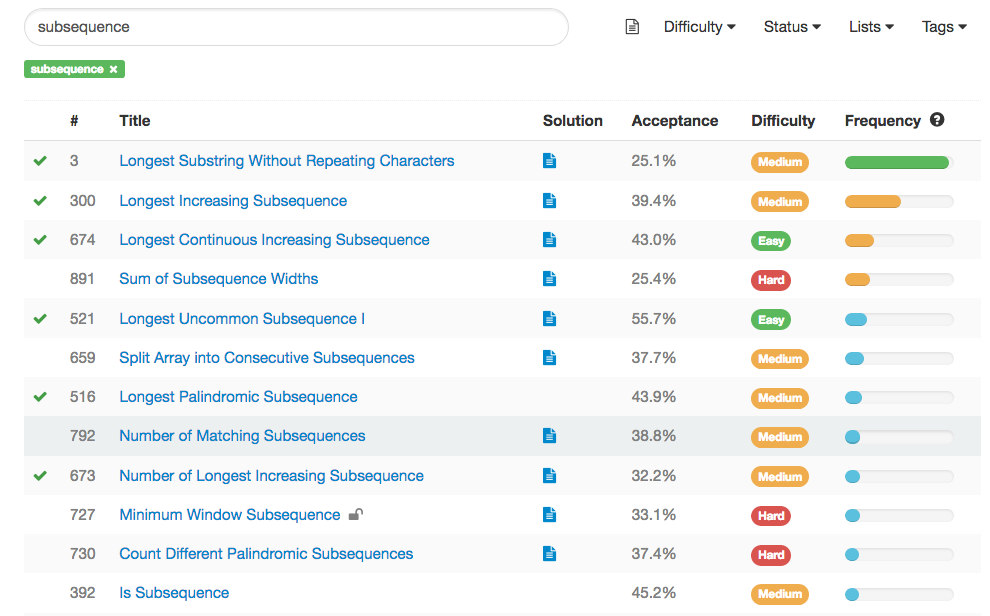
\includegraphics[width=0.8\columnwidth]{fig/subsequence_1.png}
    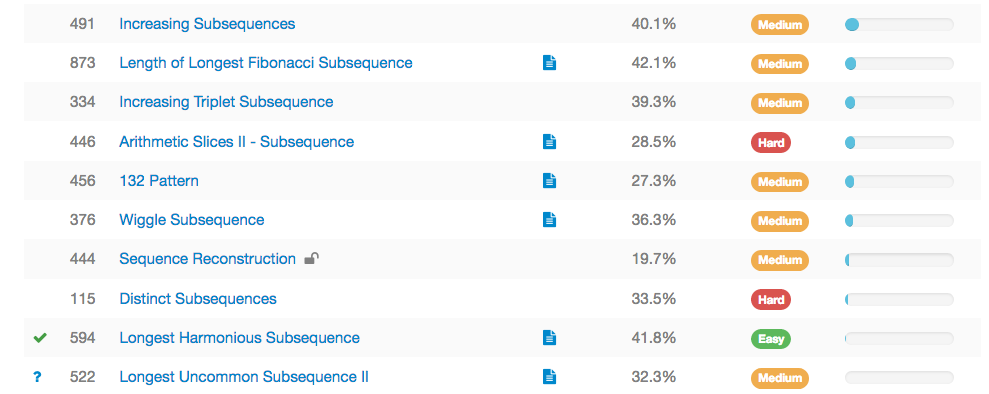
\includegraphics[width=0.8\columnwidth]{fig/subsequence_2.png}
    \caption{Subsequence Problems Listed on LeetCode}
    \label{fig:subsequence_problems}
\end{figure}
940. Distinct Subsequences II (hard)

Given a string S, count the number of distinct, non-empty subsequences of S . Since the result may be large, return the answer modulo $10^9 + 7$.
\begin{lstlisting}
Example 1:

Input: "abc"
Output: 7
Explanation: The 7 distinct subsequences are "a", "b", "c", "ab", "ac", "bc", and "abc".

Example 2:

Input: "aba"
Output: 6
Explanation: The 6 distinct subsequences are "a", "b", "ab", "ba", "aa" and "aba".

Example 3:

Input: "aaa"
Output: 3
Explanation: The 3 distinct subsequences are "a", "aa" and "aaa".
\end{lstlisting}
\textbf{Sequence type dynamic programming}. The naive solution for subsequence is using DFS to generate all of the subsequence recursively and we also need to check the repetition. The possible number of subsequence is $2^n-1$. Let's try forward induction method. 
\begin{lstlisting}
# define the result for each state: number of subsequence ends with each state
state:  a   b  c
ans  :  1   2  4 
a: a; dp[0] = 1
b: b, ab; = dp[0]+1 if this is 'a', length 1 is the same as dp[0], only length 2 is possible
c: c, ac, bc, abc; = dp[0]+dp[1]+1, if it is 'a', aa, ba, aba,  = dp[1]+1
d: d, ad, bd, abd, cd, acd, bcd, abcd = dp[0]+dp[1]+dp[2]+1
\end{lstlisting}
Thus the recurrence function can be Eq.~\ref{eq:distinct_subsequence}.
\begin{equation}
\label{eq:distinct_subsequence}
    dp[i] = \sum_{j<i}(dp[j]) +1, S[j] != S[i]
\end{equation}
Thus, we have $O(n^2)$ time complexity, and the following code:
\begin{lstlisting}[language=Python]
def distinctSubseqII(self, S):
    """
    :type S: str
    :rtype: int
    """
    MOD = 10**9+7
    dp = [1]*len(S) #means for that length it has at least one count
    for i, c in enumerate(S):
        for j in range(i):
            if c == S[j]:
                continue
            else:
                dp[i] += dp[j]
                dp[i] %= MOD
    return sum(dp) % MOD
\end{lstlisting}
However, we still get LTE. How to improve it further. If we use a counter indexed by all of the 26 letters, and a prefix sum. The inner for loop can be replaced by dp[i] = 1+ (prefix sum - sum of all S[i]).Thus we can lower the complexity further to $O(n)$.
\begin{lstlisting}[language=Python]
def distinctSubseqII(self, S):
    MOD = 10**9+7
    dp = [1]*len(S) #means for that length it has at least one count
    sum_tracker = [0]*26
    total = 0
    for i, c in enumerate(S):
        index = ord(c) - ord('a')
        dp[i] += total-sum_tracker[index]
        total += dp[i]
        sum_tracker[index] += dp[i]
    return sum(dp) % MOD
\end{lstlisting}

%%%%%%%%%%%%%%%%%%%%%%%%%%%%%%%%%%%%%%%%%%%%%%%%%%%%%%%%%%%%%%%%%%%%%%%%%%%
%%%%% Sum
%%%%%%%%%%%%%%%%%%%%%%%%%%%%%%%%%%%%%%%%%%%%%%%%%%%%%%%%%%%%%%%%%%%%%%%%%%%
% \subsection{Sum}
% In this section, to get sum we can choose to use hashmap to save the original list so that for the last element, we only check the hashmap, we can lower the complexity by one power of n. However, a better solution is to use two pointers or three pointers. for three pointers, the first one is to make sure the starting point. Also, we can think about divide and conquer.
% \begin{lstlisting}
% [-4,-1,-1,0,1,2]
% i, l-> ``````<-r
% \end{lstlisting}

% \begin{enumerate}
%     \item 
%%%%%%%%%%%%%%%%%%%%%%%%%%%%%%%%%%%%%%%%%%%%%%%%%%%%%%%%%%%%%%%%%%%%%%%%%%%
%%%%% Others
%%%%%%%%%%%%%%%%%%%%%%%%%%%%%%%%%%%%%%%%%%%%%%%%%%%%%%%%%%%%%%%%%%%%%%%%%%%
\subsection{Others}
For example, the following question would be used as follow up for question \textit{Longest Continuous Increasing Subsequence}

300. Longest Increasing Subsequence


673. Number of Longest Increasing Subsequence

Given an unsorted array of integers, find the number of longest increasing subsequence.
\begin{lstlisting}
Example 1:

Input: [1,3,5,4,7]
Output: 2
Explanation: The two longest increasing subsequence are [1, 3, 4, 7] and [1, 3, 5, 7].

Example 2:
Input: [2,2,2,2,2]
Output: 5
Explanation: The length of longest continuous increasing subsequence is 1, and there are 5 subsequences' length is 1, so output 5.
\textit{Note: Length of the given array will be not exceed 2000 and the answer is guaranteed to be fit in 32-bit signed int.}
\end{lstlisting}

Solution: Another different problem, to count the number of the max subsequence. Typical dp:

state: f[i]
\begin{lstlisting}[language = Python]
from sys import maxsize
class Solution:
    def findNumberOfLIS(self, nums):
        """
        :type nums: List[int]
        :rtype: int
        """
        max_count = 0
        if not nums:
            return 0
        memo =[None for _ in range(len(nums))]
        rlst=[]
        def recursive(idx,tail,res):
            if idx==len(nums):
                rlst.append(res)
                return 0
            if memo[idx]==None:
                length = 0
                if nums[idx]>tail:
                    addLen = 1+recursive(idx+1, nums[idx],res+[nums[idx]])
                    notAddLen = recursive(idx+1, tail,res)
                    return max(addLen,notAddLen)
                else:
                    return recursive(idx+1, tail,res)
        
        
        ans=recursive(0,-maxsize,[])
        count=0
        for lst in rlst:
            if len(lst)==ans:
                count+=1
                
        return count
\end{lstlisting}

Using dynamic programming, the difference is we add a count array.
\begin{lstlisting}[language = Python]
from sys import maxsize
class Solution:
    def findNumberOfLIS(self, nums):
        N = len(nums)
        if N <= 1: return N
        lengths = [0] * N #lengths[i] = longest ending in nums[i]
        counts = [1] * N #count[i] = number of longest ending in nums[i]

    for idx, num in enumerate(nums): #i
            for i in range(idx): #j
                if nums[i] < nums[idx]: #bigger 
                    if lengths[i] >= lengths[idx]:
                        lengths[idx] = 1 + lengths[i] #set the biggest length
                        counts[idx] = counts[i] #change the count
                    elif lengths[i] + 1 == lengths[idx]: #if it is a tie
                        counts[idx] += counts[i] #increase the current count by count[i]

longest = max(lengths)
        print(counts)
        print(lengths)
        return sum(c for i, c in enumerate(counts) if lengths[i] == longest)
\end{lstlisting}

128. Longest Consecutive Sequence
\begin{lstlisting}
Given an unsorted array of integers, find the length of the longest consecutive elements sequence.

For example,
 Given [100, 4, 200, 1, 3, 2],
 The longest consecutive elements sequence is [1, 2, 3, 4]. Return its length: 4.
 
 Your algorithm should run in O(n) complexity.
 \end{lstlisting}

Solution: Not thinking about the O(n) complexity, we can use sorting to get [1,2,3,4,100,200], and then use two pointers to get [1,2,3,4].

How about O(n)? We can pop out a number in the list, example, 4 , then we use while first-1 to get any number that is on the left side of 4, here it is 3, 2, 1, and use another to find all the bigger one and remove these numbers from the nums array.
\begin{lstlisting}[language =Python]
def longestConsecutive(self, nums):
        nums = set(nums)
        maxlen = 0
        while nums:
            first = last = nums.pop()
            while first - 1 in nums: #keep finding the smaller one
                first -= 1
                nums.remove(first)
            while last + 1 in nums: #keep finding the larger one
                last += 1
                nums.remove(last)
            maxlen = max(maxlen, last - first + 1)
        return maxlen
\end{lstlisting}


% subset
%\subfile{chapters/mastering/array/subset.tex}
%%%%%%%%%%%%%%%%%%%%%%%%%%%%%%%%%%%%%%%%%%%%%%%%%%%%%%%%%%%%%%%%%%%%%%%%%%%
%%%%% Subset
%%%%%%%%%%%%%%%%%%%%%%%%%%%%%%%%%%%%%%%%%%%%%%%%%%%%%%%%%%%%%%%%%%%%%%%%%%%
\section{Subset(Combination and Permutation)}
\label{part4_array_subset}
The Subset B of a set A is defined as a set within all elements of this subset are from set A. In other words, the subset B is contained inside the set A, $B \in A$. There are two kinds of subsets: if the order of the subset doesnt matter, it is a combination problem, otherwise, it is a permutation problem. To solve the problems in this section, we need to refer to the backtracking in Sec~\ref{sec_combination}. When the subset has a fixed constant length, then hashmap can be used to lower the complexity by one power of n.

\textbf{Subset VS Subsequence}. In the subsequence, the elements keep the original order from the original sequence. While, in the set concept, there is no ordering, only a set of elements. 

In this type of questions, we are asked to return subsets of a list. For this type of questions, backtracking~\ref{sec:backtrack} can be applied. 
\subsection{Combination}
\label{part4_array_combine}
The solution of this section is heavily correlated to Section~\ref{sec_combination}. 
78. Subsets
\begin{lstlisting}
Given a set of distinct integers, nums, return all possible subsets (the power set).

Note: The solution set must not contain duplicate subsets.

Example:

Input: nums = [1,2,3]
Output:
[
  [3],
  [1],
  [2],
  [1,2,3],
  [1,3],
  [2,3],
  [1,2],
  []
]
\end{lstlisting}
\textbf{Backtracking}. This is a combination problem, which we have explained in backtrack section. We just directly gave the code here. 
\begin{lstlisting}[language = Python]
def subsets(self, nums):
    res, n = [], len(nums)
    res = self.combine(nums, n, n)
    return res

def combine(self, nums, n, k):
    """
    :type n: int
    :type k: int
    :rtype: List[List[int]]
    """
    def C_n_k(d, k, s, curr, ans): #d controls the degree (depth), k is controls the return level, curr saves the current result, ans is all the result
        ans.append(curr)
        if d == k: #the length is satisfied

            return
        for i in range(s, n):
            curr.append(nums[i])
            C_n_k(d+1, k, i+1, curr[:], ans) # i+1 because no repeat, make sure use deep copy curr[:]
            curr.pop()

    ans = []    
    C_n_k(0, k, 0, [], ans) 
    return ans
\end{lstlisting}
\textbf{Incremental}. Backtracking is not the only way for the above problem. There is another way to do it iterative, observe the following process. We can just keep append elements to the end of of previous results. 
\begin{lstlisting}
[1, 2, 3, 4]
l = 0, []
l = 1, for 1, []+[1], -> [1],  get powerset of [1]
l = 2, for 2, []+[2], [1]+[2], -> [2], [1, 2], get powerset of [1, 2]
l = 3, for 3, []+[3], [1]+[3], [2]+[3], [1, 2]+[3], -> [3], [1, 3], [2, 3], [1, 2, 3], get powerset of [1, 2, 3]
l = 4, for 4, []+ [4]; [1]+[4]; [2]+[4], [1, 2] +[4]; [3]+[4], [1,3]+[4],[2,3]+[4], [1,2,3]+[4], get powerset of [1, 2, 3, 4]
\end{lstlisting}
\begin{lstlisting}[language=Python]
def subsets(self, nums):
    result = [[]] #use two dimensional, which already have [] one element
    for num in nums:
        new_results = []
        for r in result:
            new_results.append(r + [num])
        result += new_results
        
    return result
\end{lstlisting}
90. Subsets II
\begin{lstlisting}
Given a collection of integers that might contain duplicates, nums, return all possible subsets (the power set).

Note: The solution set must not contain duplicate subsets.

Example:

Input: [1,2,2]
Output:
[
  [2],
  [1],
  [1,2,2],
  [2,2],
  [1,2],
  []
]
\end{lstlisting}
Analysis: Because of the duplicates, the previous superset algorithm would give repetitive subset. For the above example, we would have [1, 2] twice, and [2] twice.  If we try to modify on the previous code. We first need to sort the nums, which makes the way we check repeat easiler. Then the code goes like this:
\begin{lstlisting}[language = Python]
    def subsetsWithDup(self, nums):
        """
        :type nums: List[int]
        :rtype: List[List[int]]
        """
        nums.sort()
        result = [[]] #use two dimensional, which already have [] one element
        for num in nums:
            new_results = []
            for r in result:
                print(r)
                new_results.append(r + [num])
            for rst in new_results:
                if rst not in result: # check the repetitive
                    result.append(rst)
            
        return result
\end{lstlisting}
However, the above code is extremely inefficient because of the checking process. A better way to do this:
\begin{lstlisting}
[1, 2, 2]
l = 0, []
l = 1, for 1, []+[1]
l = 2, for 2, []+[2], [1]+[2]; []+[2, 2], [1]+[2, 2]
\end{lstlisting}
So it would be more efficient if we first save all the numbers in the array in a dictionary. For the above case, the dic = {1:1, 2:2}. Each time we try to generate the result, we use 2 up to 2 times. Same way, we can use dictionary on the backtracking too. 
\begin{lstlisting}[language=Python]
class Solution(object):
    def subsetsWithDup(self, nums):
        """
        :type nums: List[int]
        :rtype: List[List[int]]
        """
        if not nums:
            return [[]]
        res = [[]]
        dic = collections.Counter(nums)
        for key, val in dic.items():
            tmp = []
            for lst in res:
                for i in range(1, val+1):
                    tmp.append(lst+[key]*i)
            res += tmp
        return res
\end{lstlisting}

77. Combinations
\begin{lstlisting}
Given two integers n and k, return all possible combinations of k numbers out of 1 ... n.

Example:

Input: n = 4, k = 2
Output:
[
  [2,4],
  [3,4],
  [2,3],
  [1,2],
  [1,3],
  [1,4],
]
\end{lstlisting}
Analysis: In this problem, it is difficult for us to generate the results iteratively, the only way we can use the second solution is by filtering and get only the results with the length we want. However, the backtrack can solve the problem easily as we mentioned in Section~\ref{sec_combination}.
\begin{lstlisting}[language=Python]
def combine(self, n, k):
    """
    :type n: int
    :type k: int
    :rtype: List[List[int]]
    """
    ans = []
    def C_n_k(d,k,s,curr):
        if d==k:
            ans.append(curr)
            return
        for i in range(s, n):
            #curr.append(i+1)
            #C_n_k(d+1, k, i+1, curr[:])
            #curr.pop()
            C_n_k(d+1, k, i+1, curr+[i+1])
    C_n_k(0,k,0,[]) 

    return ans
\end{lstlisting}
%%%%%%%%%%%%%%%%%%%combination sum%%%%%%%%%%%%%%%%%%%%%%%%%%%%
\subsection{Combination Sum}
39. Combination Sum

Given a set of candidate numbers (candidates) \textbf{(without duplicates)} and a target number (target), find all unique combinations in candidates where the candidate numbers sums to target.

The same repeated number may be chosen from candidates \textbf{unlimited number} of times.
\begin{lstlisting}
Note:

    All numbers (including target) will be positive integers.
    The solution set must not contain duplicate combinations.

Example 1:

Input: candidates = [2,3,6,7], target = 7,
A solution set is:
[
  [7],
  [2,2,3]
]

Example 2:

Input: candidates = [2,3,5], target = 8,
A solution set is:
[
  [2,2,2,2],
  [2,3,3],
  [3,5]
]
\end{lstlisting}
\textbf{DFS Backtracking}. Analysis: This is still a typical combination problem, the only thing is the return level is when the sum of the path we gained is larger than the target, and we only collect the answer when it is equal. And Because a number can be used unlimited times, so that each time after we used one number, we do not increase the next start position. 
\begin{lstlisting}[language=Python]
def combinationSum(self, candidates, target):
    """
    :type candidates: List[int]
    :type target: int
    :rtype: List[List[int]]
    """
    ans = []
    candidates.sort()
    self.combine(candidates, target, 0, [], ans)
    return ans

def combine(self, nums, target, s, curr, ans):
    if target < 0:
        return  # backtracking
    if target == 0:
        ans.append(curr)
        return 
    for i in range(s, len(nums)):
        # if nums[i] > target:
        #     return
        self.combine(nums, target-nums[i], i, curr+[nums[i]], ans) # use i, instead of i+1 because we can reuse
\end{lstlisting}
40. Combination Sum II

Given a collection of candidate numbers \textbf{(candidates with duplicates)} and a target number (target), find all unique combinations in candidates where the candidate numbers sums to target.

Each number in candidates may only \textbf{be used once} in the combination.
\begin{lstlisting}
Note:

    All numbers (including target) will be positive integers.
    The solution set must not contain duplicate combinations.

Example 1:

Input: candidates = [10,1,2,7,6,1,5], target = 8,
A solution set is:
[
  [1, 7],
  [1, 2, 5],
  [2, 6],
  [1, 1, 6]
]

Example 2:

Input: candidates = [2,5,2,1,2], target = 5,
A solution set is:
[
  [1,2,2],
  [5]
]
\end{lstlisting}
\textbf{Backtracking+Counter}. Because for the first example, if we reuse the code from the previous problem, we will get extra combinations: [7, 1], [2, 1, 5]. To avoid this, we need a dictionary to save all the unique candidates with its corresponding appearing times. For a certain number, it will be used at most its counter times. 
\begin{lstlisting}[language=Python]
def combinationSum2(self, candidates, target):
    """
    :type candidates: List[int]
    :type target: int
    :rtype: List[List[int]]
    """
        
    candidates = collections.Counter(candidates)
    ans = []
    self.combine(list(candidates.items()), target, 0, [], ans) # convert the Counter to a list of (key, item) tuple
    return ans
    
def combine(self, nums, target, s, curr, ans):
    if target < 0:
        return 
    if target == 0:
        ans.append(curr)
        return
    for idx in range(s, len(nums)):           
        num, count = nums[idx]
        for c in range(count):
            self.combine(nums, target-num*(c+1), idx+1, curr+[num]*(c+1), ans )
\end{lstlisting}
377. Combination Sum IV (medium)
\begin{lstlisting}
 Given an integer array with all positive numbers and no duplicates, find the number of possible combinations that add up to a positive integer target.

Example:

nums = [1, 2, 3]
target = 4

The possible combination ways are:
(1, 1, 1, 1)
(1, 1, 2)
(1, 2, 1)
(1, 3)
(2, 1, 1)
(2, 2)
(3, 1)

Note that different sequences are counted as different combinations.

Therefore the output is 7.

Follow up:
What if negative numbers are allowed in the given array?
How does it change the problem?
What limitation we need to add to the question to allow negative numbers? 
\end{lstlisting}
\textbf{DFS + MEMO}. This problem is similar to 39. Combination Sum. For [2, 3, 5], target = 8,  comparison:
\begin{lstlisting}
[2, 3, 5], target = 8
39. Combination Sum. # there is ordering (each time the start index is same or larger than before)
[
  [2,2,2,2],
  [2,3,3],
  [3,5]
]
377. Combination Sum IV, here we have no ordering( each time the start index is the same as before). Try all element.
[
  [2,2,2,2],
  [2,3,3],
* [3,3,2]
* [3,2,3]
  [3,5],
* [5,3]
]
\end{lstlisting}
\begin{lstlisting}[language=Python]
def combinationSum4(self, nums, target):
    """
    :type nums: List[int]
    :type target: int
    :rtype: int
    """
    nums.sort()
    n = len(nums)
    def DFS(idx, memo, t):
        if t < 0:
            return 0
        if t == 0:
            return 1
        count = 0
        if t not in memo:
            for i in range(idx, n):
                count += DFS(idx, memo, t-nums[i])
            memo[t] = count
        return memo[t]
    return(DFS(0, {}, target))
\end{lstlisting}
Because, here we does not need to numerate all the possible solutions, we can use dynamic programming, which will be shown in Section~\ref{}. 

\subsection{K Sum}
In this subsection, we still trying to get subset that sum up to a target. But the length here is fixed. We would have 2, 3, 4 sums normally. Because it is still a combination problem, we can use the \textbf{backtracking} to do. Second, because the fixed length, we can use \textbf{multiple pointers} to build up the potential same lengthed subset.  But in some cases, because the length is fixed, we can use \textbf{hashmap} to simplify the complexity. 

1. Two Sum
Given an array of integers, return \textbf{indices} of the two numbers such that they add up to a specific target.

You may assume that each input would have \textbf{exactly} one solution, and you may not use the same element twice.
\begin{lstlisting}
Example:

Given nums = [2, 7, 11, 15], target = 9,

Because nums[0] + nums[1] = 2 + 7 = 9,
return [0, 1].
\end{lstlisting}
\textbf{Hashmap}. Using backtracking or brute force will get us $O(n^2)$ time complexity. We can use hashmap to save the nums in a dictionary. Then we just check target-num in the dictionary. We would get $O(n)$ time complexity. We have two-pass hashmap and one-pass hashmap.
\begin{lstlisting}[language=Python]
# two-pass hashmap
def twoSum(self, nums, target):
    """
    :type nums: List[int]
    :type target: int
    :rtype: List[int]
    """
    dict = collections.defaultdict(int)
    for i, t in enumerate(nums):
        dict[t] = i
    for i, t in enumerate(nums):
        if target - t in dict and i != dict[target-t]:
            return [i, dict[target-t]]
# one-pass hashmap
def twoSum(self, nums, target):
    """
    :type nums: List[int]
    :type target: int
    :rtype: List[int]
    """
    dict = collections.defaultdict(int)
    for i, t in enumerate(nums):
        if target - t in dict:
            return [dict[target-t], i]
        dict[t] = i
\end{lstlisting}

15. 3Sum

Given an array S of n integers, are there elements a, b, c in S such that a + b + c = 0? Find all unique triplets in the array which gives the sum of zero.

Note: The solution set must not contain duplicate triplets.

For example, given array S = [-1, 0, 1, 2, -1, -4],
\begin{lstlisting}
A solution set is:
[
  [-1, 0, 1],
  [-1, -1, 2]
]
\end{lstlisting}

Solution: Should use three pointers, no extra space. i is the start point from [0,len-2], l,r is the other two pointers. l=i+1, r=len-1 at the beignning. The saving of time complexity is totally from the sorting algorithm.
\begin{lstlisting}
[-4,-1,-1,0,1,2]
i, l-> ``````<-r
\end{lstlisting}
How to delete repeat?
\begin{lstlisting}[language = Python]
def threeSum(self, nums):
    res = []
    nums.sort()
    for i in xrange(len(nums)-2):
        if i > 0 and nums[i] == nums[i-1]: #make sure pointer not repeat
            continue
        l, r = i+1, len(nums)-1
        while l < r:
            s = nums[i] + nums[l] + nums[r]
            if s < 0:
                l +=1 
            elif s > 0:
                r -= 1
            else:
                res.append((nums[i], nums[l], nums[r]))
                l+=1
                r-=1

                #after the first run, then check duplicate example.
                while l < r and nums[l] == nums[l-1]:
                    l += 1
                while l < r and nums[r] == nums[r+1]:
                    r -= 1
    return res
\end{lstlisting}
Use hashmap:
\begin{lstlisting}[language = Python]
def threeSum(self, nums):
        """
        :type nums: List[int]
        :rtype: List[List[int]]
        """
        res =[]
        nums=sorted(nums)
        if not nums:
            return []
        if nums[-1]<0 or nums[0]>0:
            return []
        end_position = len(nums)-2
        dic_nums={}
        for i in xrange(1,len(nums)):
            dic_nums[nums[i]]=i# same result save the last index
        
        for i in xrange(end_position):
            target = 0-nums[i]
            if i>0 and nums[i] == nums[i-1]: #this is to avoid repeat 
                continue
            if target<nums[i]: #if the target is smaller than this, we can not find them on the right side
                break
            for j in range(i+1,len(nums)): #this is to avoid repeat 
                if j>i+1 and nums[j]==nums[j-1]:
                    continue
                complement =target - nums[j]
                if complement<nums[j]: #if the left numbers are bigger than the complement, no need to keep searching
                    break
                if complement in dic_nums and dic_nums[complement]>j: #need to make sure the complement is bigger than nums[j]
                    res.append([nums[i],nums[j],complement])
        return res
\end{lstlisting}
The following code uses more time
\begin{lstlisting}[language = Python]
for i in xrange(len(nums)-2):
            if i > 0 and nums[i] == nums[i-1]:
                continue
            l, r = i+1, len(nums)-1
            while l < r:
                if l-1>=i+1 and nums[l] == nums[l-1]: #check the front
                    l += 1
                    continue
                if r+1<len(nums) and nums[r] == nums[r+1]:
                    r -= 1
                    continue
                s = nums[i] + nums[l] + nums[r]
                if s < 0:
                    l +=1 
                elif s > 0:
                    r -= 1
                else:
                    res.append((nums[i], nums[l], nums[r]))
                    l += 1; r -= 1
        return res
\end{lstlisting}
18. 4Sum
\begin{lstlisting}[language = Python]
def fourSum(self, nums, target):
        def findNsum(nums, target, N, result, results):
            if len(nums) < N or N < 2 or target < nums[0]*N or target > nums[-1]*N:  # early termination
                return
            if N == 2: # two pointers solve sorted 2-sum problem
                l,r = 0,len(nums)-1
                while l < r:
                    s = nums[l] + nums[r]
                    if s == target:
                        results.append(result + [nums[l], nums[r]])
                        l += 1
                        r-=1
                        while l < r and nums[l] == nums[l-1]:
                            l += 1
                        while l < r and nums[r] == nums[r+1]:
                            r -= 1
                    elif s < target:
                        l += 1
                    else:
                        r -= 1
            else: # recursively reduce N
                for i in range(len(nums)-N+1):
                    if i == 0 or (i > 0 and nums[i-1] != nums[i]):
                        findNsum(nums[i+1:], target-nums[i], N-1, result+[nums[i]], results) #reduce nums size, reduce target, save result

results = []
        findNsum(sorted(nums), target, 4, [], results)
        return results
\end{lstlisting}

454. 4Sum II

Given four lists A, B, C, D of integer values, compute how many tuples (i, j, k, l) there are such that A[i] + B[j] + C[k] + D[l] is zero.

To make problem a bit easier, all A, B, C, D have same length of N where $0 \leq N \leq 500$. All integers are in the range of -228 to 228–1 and the result is guaranteed to be at most 231–1.

Example:
\begin{lstlisting}
Input:
A = [ 1, 2]
B = [-2,-1]
C = [-1, 2]
D = [ 0, 2]

Output:
2
\end{lstlisting}

Explanation:

\begin{lstlisting}
The two tuples are:
1. (0, 0, 0, 1) -> A[0] + B[0] + C[0] + D[1] = 1 + (-2) + (-1) + 2 = 0
2. (1, 1, 0, 0) -> A[1] + B[1] + C[0] + D[0] = 2 + (-1) + (-1) + 0 = 0
\end{lstlisting}
Solution: if we use brute force, use 4 for loop, then it is $O(N^4)$. If we use divide and conquer, sum the first half, and save a dictionary (counter), time complexity is $O(2N^2)$. What if we have 6 sum, we can reduce it to $O(2N^3)$, what if 8 sum.

\begin{lstlisting}[language = Python]
def fourSumCount(self, A, B, C, D):
    AB = collections.Counter(a+b for a in A for b in B)
    return sum(AB[-c-d] for c in C for d in D)
\end{lstlisting}


\subsubsection{Summary}
As we have seen from the shown examples in this section, to solve the combination problem, backtrack shown in Section~\ref{sec_combination} offers a universal solution. Also, there is another iterative solution which suits the power set purpose. And I would include its code here again:
\begin{lstlisting}[language = Python]
def subsets(self, nums):
    result = [[]] #use two dimensional, which already have [] one element
    for num in nums:
        new_results = []
        for r in result:
            new_results.append(r + [num])
        result += new_results
        
    return result
\end{lstlisting}
If we have duplicates, how to handle in the backtrack?? In the iterative solution, we can replace the array with a dictionary saves the counts. 

\subsection{Permutation}
46. Permutations
\begin{lstlisting}
Given a collection of distinct numbers, return all possible permutations.

For example,
 [1,2,3] have the following permutations:

[
  [1,2,3],
  [1,3,2],
  [2,1,3],
  [2,3,1],
  [3,1,2],
  [3,2,1]
]
\end{lstlisting}

47. Permutations II

Given a collection of numbers that might contain duplicates, return all possible unique permutations.

For example,
\begin{lstlisting}
 [1,1,2] have the following unique permutations:

[
  [1,1,2],
  [1,2,1],
  [2,1,1]
]
\end{lstlisting}

301. Remove Invalid Parentheses

Remove the minimum number of invalid parentheses in order to make the input string valid. Return all possible results.

Note: The input string may contain letters other than the parentheses ( and ).

Examples:
\begin{lstlisting}
"()())()" -> ["()()()", "(())()"]
"(a)())()" -> ["(a)()()", "(a())()"]
")(" -> [""]
\end{lstlisting}


%%%%%%%%%%%%%%%%%%%%%%%%%%%%%%%%%%%%%%%%%%%%%%%%%%%%%%%%%%%%%%%%%%%%%%%%%%%
%%%%% Merge List
%%%%%%%%%%%%%%%%%%%%%%%%%%%%%%%%%%%%%%%%%%%%%%%%%%%%%%%%%%%%%%%%%%%%%%%%%%%
\section{Merge and Partition}
\subsection{Merge Lists}
We can use divide and conquer (see the merge sort) and the priority queue.
\subsection{Partition Lists}
Partition of lists can be converted to subarray, combination, subsequence problems. For example, 
\begin{enumerate}
    \item 416. Partition Equal Subset Sum (combination)
    \item 698. Partition to K Equal Sum Subsets
\end{enumerate} 

%%%%%%%%%%%%%%%%%%%%%%%%%%%%%%%%%%%%%%%%%%%%%%%%%%%%%%%%%%%%%%%%%%%%%%%%%%%%%%%%%%%%%
%%%%%%%%%%%%% Sweep Line
%%%%%%%%%%%%%%%%%%%%%%%%%%%%%%%%%%%%%%%%%%%%%%%%%%%%%%%%%%%%%%%%%%%%%%%%%%%%%%%%%%%%%%%%%
\section{Intervals}
\label{sec_sweep_line}
% \documentclass[../../main.tex]{subfiles}
Sweep Line is a type of algorithm that mainly used to solve problems with intervals of one-dimensional. Let us look at one example:
1. 253. Meeting Rooms II

Given an array of meeting time intervals consisting of start and end times [[s1,e1],[s2,e2],...] (si < ei), find the minimum number of conference rooms required.
\begin{lstlisting}
Example 1:

Input: [[0, 30],[5, 10],[15, 20]]
Output: 2

Example 2:

Input: [[7,10],[2,4]]
Output: 1
\end{lstlisting}
It would help a lot if at first we can draw one example with cooridinates.
\begin{figure}[h]
    \centering
    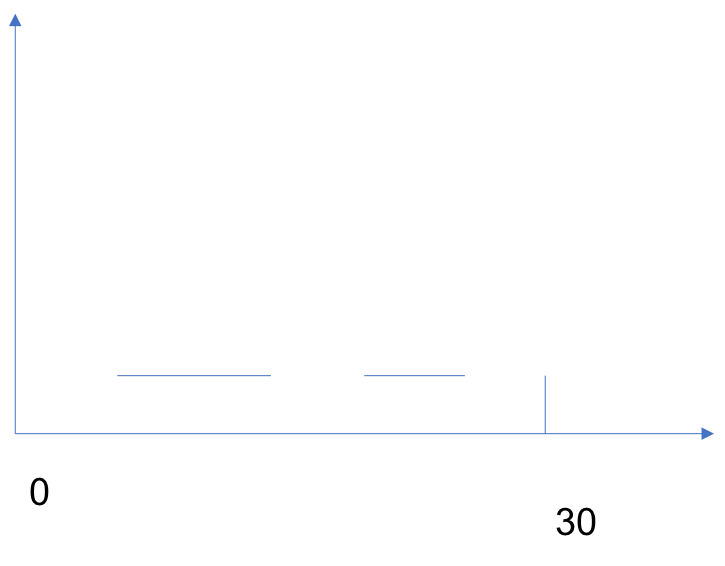
\includegraphics[width = 0.6\columnwidth]{fig/sweep_line_253.png}
    \caption{Interval questions}
    \label{fig:interval}
\end{figure}
First, the simplest situation is when we only need one meeting room is there is no intersection between these time intervals. If we add one interval that only intersect with one of the previous intervals, this means we need two conference rooms. So to find the minimum conference rooms we need, we need to find the maximum number of intersection between these time intervals. The most native solution is to scan all the time slot in one for loop, and at another inner loop go through all the intervals, if this time slot is in this intervals, then we increase the minimum number of meeting room counter. This gives us time complexity of $O(n*m)$, where $n$ is the number of intervals and $m$ is the total number of time slots. The Python code is as follows, unfortunately, with this solution we have LTE error.  
\begin{lstlisting}[language = Python]
# Definition for an interval.
# class Interval(object):
#     def __init__(self, s=0, e=0):
#         self.start = s
#         self.end = e

from collections import defaultdict
from heapq import heappush, heappop
from sys import maxint
class Solution(object):
    def minMeetingRooms(self, intervals):
        """
        :type intervals: List[Interval]
        :rtype: int
        """
        if not intervals:
            return 0
        #solution 1, voting, time complexity is O(e1-s1), 71/77 test, TLE
        votes = defaultdict(int)
        num_rooms = 0   
        for interval in intervals:
            s=interval.start
            e=interval.end
            for i in range(s+1,e+1):
                votes[i]+=1
                num_rooms = max(num_rooms, votes[i])
        return num_rooms
\end{lstlisting}
\subsection{Speedup with Sweep Line}
Now, let us see how to speed up this process. We can use Sweep Line method. For the sweep line, we have three basic implementations: one-dimensional, min-heap, or map based. 
\subsubsection{One-dimensional Implementation}
 To get the maximum number of intersection of all the intervals, it is not necessarily to scan all the time slots, how about just scan the key slot: the starts and ends . Thus, what we can do is to open an array and put all the start or end slot into the array, and with $1$ to mark it as start and $0$ to mark it as end. Then we sort this array. Till this point, how to get the maximum intersection? We go through this sorted array, if we get a start our current number of room needed will increase by one, otherwise, if we encounter an end slot, it means one meeting room is freed, thus we decrease the current on-going meeting room by one. We use another global variable to track the maximum number of rooms needed in this whole process. Great, because now our time complexity is decided by the number of slots $2n$, with the sorting algorithm, which makes the whole time complexity $O(nlogn)$ and space complexity $n$. This speeded up algorithm is called Sweep Line algorithm. Before we write our code, we better check the \textit{special cases}, what if there is one slot that is marked as start in one interval but is the end of another interval. This means we can not increase the counting at first, but we need to decrease, so that the sorting should be based on the first element of the tuple, and followed by the second element of the tuple. For example, the simple case $[[13,15],[1,13]]$, we only need maximum of one meeting room. Thus it can be implemented as:
\begin{figure}[h]
    \centering
    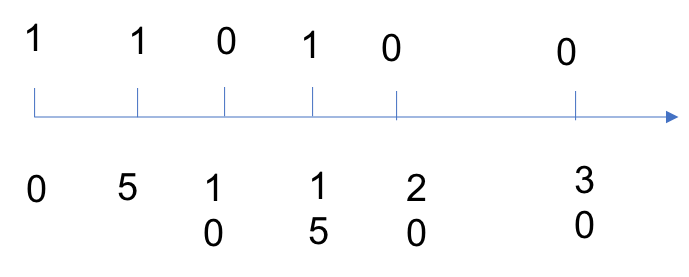
\includegraphics[width=0.6\columnwidth]{fig/sweep_line_one_dimension.png}
    \caption{One-dimensional Sweep Line}
    \label{fig:one_dim_sl}
\end{figure}
\begin{lstlisting}[language=Python]
 def minMeetingRooms(self, intervals):
        if not intervals:
            return 0       
        #solution 2
        slots = []
        # put slots into one-dimensional axis
        for i in intervals:
            slots.append((i.start, 1))
            slots.append((i.end, 0))
        # sort these slots on this dimension
        #slots.sort(key = lambda x: (x[0], x[1]))
        slots.sort()
        
        # now execute the counting
        crt_room, max_room = 0, 0
        for s in slots:
            if s[1]==0: # if it ends, decrease
                crt_room-=1
            else:
                crt_room+=1
            max_room = max(max_room, crt_room)
        return max_room
\end{lstlisting}
\subsubsection{Min-heap Implementation}
\begin{figure}[h]
    \centering
    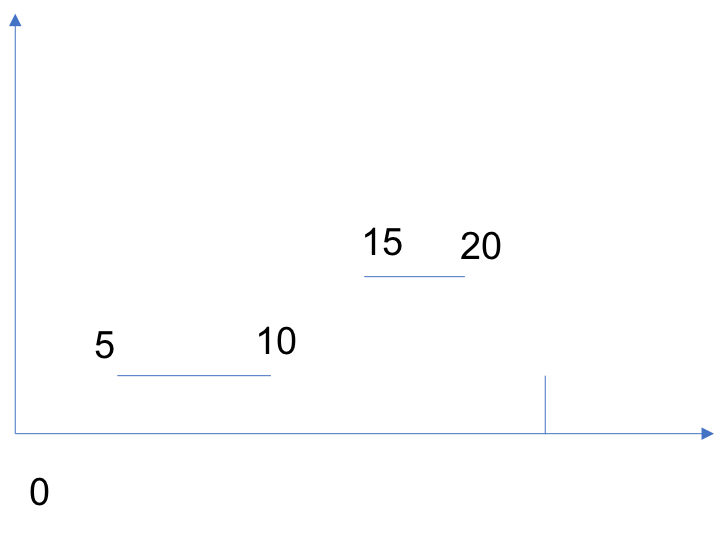
\includegraphics[width=0.6\columnwidth]{fig/sweep_line_min_heap.png}
    \caption{Min-heap for Sweep Line}
    \label{fig:min_heap_sl}
\end{figure}
Instead of opening an array to save all the time slots, we can directly sort the intervals in the order of the start time. We can see Fig.~\ref{fig:min_heap_sl}, we go through the intervals and visit their end time, the first one we encounter is $30$, we put it in a min-heap, and then we visit the next interval $[5, 10]$, $5$ is smaller than the previous end time $30$, it means this interval intersected with a previous interval, so the number of maximum rooms increase $1$, we get $2$ rooms now. We put $10$ into the min-heap. Next, we visit $[15, 20]$, $15$ is larger than the first element in the min-heap $10$, it means that these two intervals can be merged into one $[5, 20]$, so we need to update the end time $10$ to $20$. 

This way, the time complexity is still the same which is decided by the sorting algorithm. While the space complexity is decided by real situation, it varies from $O(1)$ (no intersection) to $O(n)$ (all the meetings are intersected at at least one time slot).  
\begin{lstlisting}[language=Python]
def minMeetingRooms(self, intervals):
        if not intervals:
            return 0
        #solution 2
        intervals.sort(key=lambda x:x.start)
        h = [intervals[0].end]
        rooms = 1
        for i in intervals[1:]:
            s,e=i.start, i.end
            e_before = h[0]
            if s<e_before: #overlap
                heappush(h, i.end)
                rooms+=1
            else: #no overlap
                #merge
                heappop(h) #kick out 10 in our example
                heappush(h,e) # replace 10 with 20
        return rooms
\end{lstlisting}
% 2、multiset:这次是先对每个区间的起点排序,然后依次将每个区间的终点放在一个集合中。如果下一个区间的起点大于等于之前某个区间的终点,就将其从集合中删除,每次需要统计一下当前所需的最大办公室数量。这个版本的时间复杂度还是O(nlogn),但是空间复杂度却变成output-dependent的了,最多是O(n),最少是O(1)。
\subsubsection{Map-based Implementation}

% 3、map:我们用一个map来存储重合区域,即每个区间的起点代表一个区间的开始,会将重叠区域+1,每个区间的结束点代表一个区间的结束,会将重叠区域-1。因此我们可以利用这个性质,结合STL中的map来实现(实质上这个算法和“一维向量”版本非常像,只是采用的数据结构不同而已)。
% --------------------- 
% 作者:魔豆Magicbean 
% 来源:CSDN 
% 原文:https://blog.csdn.net/magicbean2/article/details/74199529 
% 版权声明:本文为博主原创文章,转载请附上博文链接!

\begin{lstlisting}[language=Python]
class Solution {
public:
    int minMeetingRooms(vector<Interval>& intervals) {
        map<int, int> mp;
        for (auto val : intervals) {
            ++mp[val.start];
            --mp[val.end];
        }
        int max_room = 0, crt_room = 0;
        for (auto val : mp) {
            crt_room += val.second;
            max_room = max(max_room, crt_room);
        }
        return max_room;
    }
};
\end{lstlisting}

\subsection{LeetCode Problems}
\begin{enumerate}
 \item \textbf{986. Interval List Intersections} Given two lists of closed intervals, each list of intervals is pairwise disjoint and in sorted order. Return the intersection of these two interval lists.
\begin{lstlisting}[numbers=none]
Input: A = [[0,2],[5,10],[13,23],[24,25]], B = [[1,5],[8,12],[15,24],[25,26]]
Output: [[1,2],[5,5],[8,10],[15,23],[24,24],[25,25]]
Reminder: The inputs and the desired output are lists of Interval objects, and not arrays or lists.
\end{lstlisting}
\end{enumerate}
%%%%%%%%%%%%%%%%%%%%%%%%%%%%%%%%%%%%%%%%%%%%%%%%%%%%%%%%%%%%%%%%%%%%%%%%%%%
%%%%% Intersection
%%%%%%%%%%%%%%%%%%%%%%%%%%%%%%%%%%%%%%%%%%%%%%%%%%%%%%%%%%%%%%%%%%%%%%%%%%%
\section{Intersection}
For problems to get intersections of lists, we can use hashmap, which takes $O(m+n)$ time complexity. Also, we can use sorting at first and use two pointers one start from the start of each array. Examples are shown as below;
\begin{enumerate}
    \item  349. Intersection of Two Arrays (Easy)
    
     Given two arrays, write a function to compute their intersection.

Example:
\begin{lstlisting}
Given nums1 = [1, 2, 2, 1], nums2 = [2, 2], return [2].
\end{lstlisting}

Note:
\begin{itemize}
    \item Each element in the result must be unique.
    \item The result can be in any order.
\end{itemize}
Solution 1: Using hashmap, here we use set to convert, this takes 43ms. 
\begin{lstlisting}[language = Python]
def intersection(self, nums1, nums2):
    """
    :type nums1: List[int]
    :type nums2: List[int]
    :rtype: List[int]
    """
    if not nums1 or not nums2:
        return []
    if len(nums1) > len(nums2):
        nums1, nums2 = nums2, nums1
    ans = set()
    nums1 = set(nums1)
    for e in nums2:
        if e in nums1:
            ans.add(e)
    return list(ans)
\end{lstlisting}
Solution2: sorting at first, and then use pointers. Take 46 ms. 
\begin{lstlisting}[language = Python]
def intersection(self, nums1, nums2):
    """
    :type nums1: List[int]
    :type nums2: List[int]
    :rtype: List[int]
    """
    nums1.sort()
    nums2.sort()
    r = set()
    i, j = 0, 0
    while i < len(nums1) and j < len(nums2):
        if nums1[i] < nums2[j]:
            i += 1
        elif nums1[i] > nums2[j]:
            j += 1
        else:
            r.add(nums1[i])
            i += 1
            j += 1
    return list(r)
\end{lstlisting}
\item 350. Intersection of Two Arrays II(Easy)

 Given two arrays, write a function to compute their intersection.

Example:
\begin{lstlisting}
Given nums1 = [1, 2, 2, 1], nums2 = [2, 2], return [2, 2].
\end{lstlisting}

Note:
\begin{itemize}
    \item Each element in the result should appear as many times as it shows in both arrays.
    \item The result can be in any order.
\end{itemize}

Follow up:
\begin{enumerate}
    \item  What if the given array is already sorted? How would you optimize your algorithm?
    \item What if nums1's size is small compared to nums2's size? Which algorithm is better?
    \item What if elements of nums2 are stored on disk, and the memory is limited such that you cannot load all elements into the memory at once?
\end{enumerate}

\end{enumerate}

\section{Miscellanous Questions}
\begin{examples}[resume]
\item \textbf{283. Move Zeroes. (Easy)} 
Given an array nums, write a function to move all 0's to the end of it while maintaining the relative order of the non-zero elements.

Note:
\begin{enumerate}
    \item You must do this in-place without making a copy of the array.
    \item Minimize the total number of operations.
\end{enumerate}
\begin{lstlisting}[language=Python]
Example:

Input: [0,1,0,3,12]
Output: [1,3,12,0,0]
\end{lstlisting}
\textbf{Solution 1: Find All Zeros Subarray.} If we found the first all zeros subarray [0, ..., 0] + [x], and we can swap this subarray with the first non-zero element as swap last 0 with x, swap second last element with x, ..., and so on. Therefore, if 0 is at first index, one zero, then it takes O(n), if another 0, at index 1, it takes n-1+n-2 = 2n. It is bit tricky to compute the complexity analysis. The upper bound is $O(n^2)$. 
\end{examples}
%%%%%%%%%%%%%%%%%%%%%%%%%%%%%%%%%%%%%%%%%%%%%%%%%%%%%%%%%%%%%%%%%%%%%%%%%%%
%%%%% Exercises
%%%%%%%%%%%%%%%%%%%%%%%%%%%%%%%%%%%%%%%%%%%%%%%%%%%%%%%%%%%%%%%%%%%%%%%%%%%
\section{Exercises}
% %%%%%%%%%%%%%%%%%%%%%%%%%%%%%%%%%%%%%%%%%%%%%%%%%%%%%%%%%%%%%%%%%%%%%%%%%%%
% %%%%% Subsequence
% %%%%%%%%%%%%%%%%%%%%%%%%%%%%%%%%%%%%%%%%%%%%%%%%%%%%%%%%%%%%%%%%%%%%%%%%%%%
\subsection{Subsequence with (DP)}

\begin{enumerate}
    \item 594. Longest Harmonious Subsequence

We define a harmonious array is an array where the difference between its maximum value and its minimum value is exactly 1.

Now, given an integer array, you need to find the length of its longest harmonious subsequence among all its possible subsequences.

Example 1:
\begin{lstlisting}
Input: [1,3,2,2,5,2,3,7]
Output: 5
Explanation: The longest harmonious subsequence is [3,2,2,2,3].
\end{lstlisting}

\textit{Note: The length of the input array will not exceed 20,000.}

Solution: at first, use a Counter to save the whole set. Then visit the counter dictionary, to check key+1 and key-1, only when the item is not zero, we can count it as validate, or else it is 0.
\begin{lstlisting}[language = Python]
from collections import Counter
class Solution:
    def findLHS(self, nums):
        """
        :type nums: List[int]
        :rtype: int
        """
        if not nums or len(nums)<2:
            return 0
        count=Counter(nums) #the list is sorted by the key value
        maxLen = 0
        for key,item in count.items(): #to visit the key: item in the counter
            if count[key+1]: #because the list is sorted, so we only need to check key+1
                maxLen = max(maxLen,item+count[key+1])
            
            # if count[key-1]:
            #     maxLen=max(maxLen, item+count[key-1])
        return maxLen
\end{lstlisting}

\item 521. Longest Uncommon Subsequence I

Given a group of two strings, you need to find the longest uncommon subsequence of this group of two strings. The longest uncommon subsequence is defined as the longest subsequence of one of these strings and this subsequence should not be any subsequence of the other strings.

A subsequence is a sequence that can be derived from one sequence by deleting some characters without changing the order of the remaining elements. Trivially, any string is a subsequence of itself and an empty string is a subsequence of any string.

The input will be two strings, and the output needs to be the length of the longest uncommon subsequence. If the longest uncommon subsequence doesn’t exist, return -1.

Example 1:
\begin{lstlisting}
Input: "aba", "cdc"
Output: 3
Explanation: The longest uncommon subsequence is "aba" (or "cdc"), 
because "aba" is a subsequence of "aba", 
but not a subsequence of any other strings in the group of two strings.
\end{lstlisting}

\textit{Note:}

    \textit{Both strings’ lengths will not exceed 100.}
    
    \textit{Only letters from a ~ z will appear in input strings.}

Solution: if we get more examples, we could found the following rules, “aba”,”aba” return -1,
\begin{lstlisting}[language = Python]
def findLUSlength(self, a, b):
        """
        :type a: str
        :type b: str
        :rtype: int
        """
        if len(b)!=len(a):
            return max(len(a),len(b))
        #length is the same
        return len(a) if a!=b else -1
\end{lstlisting}
\item 424. Longest Repeating Character Replacement

Given a string that consists of only uppercase English letters, you can replace any letter in the string with another letter at most k times. Find the length of a longest substring containing all repeating letters you can get after performing the above operations.

\textit{Note:}

 \textit{Both the string’s length and k will not exceed 104.}

Example 1:
\begin{lstlisting}
Input:
s = "ABAB", k = 2

Output:
4
\end{lstlisting}

Explanation:
Replace the two 'A's with two 'B's or vice versa.

Example 2:
\begin{lstlisting}
Input:
s = "AABABBA", k = 1

Output:
4
\end{lstlisting}

Explanation:
Replace the one 'A' in the middle with 'B' and form "AABBBBA".
The substring "BBBB" has the longest repeating letters, which is 4.

Solution: the brute-force recursive solution for this, is try to replace any char into another when it is not equal or choose not too. LTE
\begin{lstlisting}[language = Python]
#brute force, use recursive function to write brute force solution
        def replace(news, idx, re_char, k):
            nonlocal maxLen
            if k==0 or idx==len(s):
                maxLen = max(maxLen, getLen(news))
                return

if s[idx]!=re_char: #replace
                news_copy=news[:idx]+re_char+news[idx+1:]
                replace(news_copy, idx+1, re_char, k-1)
            replace(news[:], idx+1, re_char,k)
        
        #what if we only have one char
        # for char1 in chars.keys():
        #     replace(s[:],0,char1, k)
\end{lstlisting}
To get the BCR, think about the sliding window. The longest repeating string we can by number of replacement = `length of string max(numer of occurence of letter i), i=’A’ to ‘Z’. With the constraint, which means the equation needs to be $\leq k$. So we can use sliding window to record the max occurence, and when the constraint is violated, we shrink the window. Given an example, strs= “BBCABBBAB”, k=2, when i=0, and j=7, 8–5=3>2, which is at A, we need to shrink it, the maxCharCount changed to 4, i=1, so that 8–1–4=3, i=2, 8–2–3=3, 8–3–3=2, so i=3, current length is 5.
\begin{lstlisting}[language = Python]
def characterReplacement(self, s, k):
        """
        :type s: str
        :type k: int
        :rtype: int
        """
        i,j = 0,0 #sliding window
        counter=[0]*26
        ans = 0
        maxCharCount = 0
        while j<len(s):
            counter[ord(s[j])-ord('A')]+=1
            maxCharCount = max(maxCharCount, counter[ord(s[j])-ord('A')])
            while j-i+1-maxCharCount>k: #now shrink the window
                counter[ord(s[i])-ord('A')]-=1
                i+=1
                #updata max
                maxCharCount=max(counter)
            ans=max(ans, j-i+1)
            j+=1
                
        return ans
\end{lstlisting}

\item 395. Longest Substring with At Least K Repeating Characters

Find the length of the longest substring T of a given string (consists of lowercase letters only) such that every character in T appears no less than k times.

Example 1:
\begin{lstlisting}
Input:
s = "aaabb", k = 3

Output:
3
\end{lstlisting}

The longest substring is "aaa", as 'a' is repeated 3 times.

Example 2:
\begin{lstlisting}
Input:
s = "ababbc", k = 2

Output:
5
\end{lstlisting}

The longest substring is "ababb", as 'a' is repeated 2 times and 'b' is repeated 3 times.

Solution: use dynamic programming with memo: Cons: it takes too much space, and with LTE.
\begin{lstlisting}[language = Python]
from collections import Counter, defaultdict
class Solution:
    def longestSubstring(self, s, k):
        """
        :type s: str
        :type k: int
        :rtype: int
        """
        if not s:
            return 0
        if len(s)<k:
            return 0
        count = Counter(char for char in s)
        print(count)
        memo=[[None for col in range(len(s))] for row in range(len(s))]

def cut(start,end,count):
            if start>end:
                return 0
            if memo[start][end]==None:
                if any(0<item<k for key,item in count.items()):
                    newCounterF=count.copy()
                    newCounterF[s[start]]-=1
                    newCounterB=count.copy()
                    newCounterB[s[end]]-=1
                    #print(newsF,newsB)
                    memo[start][end]= max(cut(start+1, end, newCounterF), cut(start, end-1, newCounterB))
                else:
                    memo[start][end] = end-start+1
            return memo[start][end]
        return cut(0,len(s)-1,count)
\end{lstlisting}

Now, use sliding window, we use a pointer mid, what start from 0, if the whole string satisfy the condition, return len(s). Otherwise, use two while loop to separate the string into three substrings: left, mid, right. left satisfy, mid unsatisfy, right unknown.
\begin{lstlisting}[language = Python]
from collections import Counter, defaultdict
class Solution:
    def longestSubstring(self, s, k):
        """
        :type s: str
        :type k: int
        :rtype: int
        """
        if not s:
            return 0
        if len(s)<k:
            return 0
        count = Counter(char for char in s)
        mid=0 #on the left side, from 0-mid, satisfied elments
        while mid<len(s) and count[s[mid]]>=k:
            mid+=1
        if mid==len(s): return len(s) 
        left = self.longestSubstring(s[:mid],k) #"ababb"
        #from pre_mid - cur_mid, get rid of those cant satisfy the condition
        while mid<len(s) and count[s[mid]]<k:
            mid+=1
        #now the right side keep doing it
        right = self.longestSubstring(s[mid:],k)
        return max(left,right)
\end{lstlisting}
\end{enumerate}

%%%%%%%%%%%%%%%%%%%%%%%%%%%%%%%%%%%%%%%%%%%%%%%%%%%%%%%%%%%%%%%%%%%%%%%%%%%
%%%%% Subset
%%%%%%%%%%%%%%%%%%%%%%%%%%%%%%%%%%%%%%%%%%%%%%%%%%%%%%%%%%%%%%%%%%%%%%%%%%%
\subsection{Subset}
\label{sec_array_subset}


216. Combination Sum III


Find all possible combinations of \textbf{k numbers} that add up to a number n, given that only numbers from 1 to 9 can be used and each combination should be a unique set of numbers.
\begin{lstlisting}[numbers=none]
Note:

    All numbers will be positive integers.
    The solution set must not contain duplicate combinations.

Example 1:

Input: k = 3, n = 7
Output: [[1,2,4]]

Example 2:

Input: k = 3, n = 9
Output: [[1,2,6], [1,3,5], [2,3,4]]
\end{lstlisting}
\begin{lstlisting}[language=Python]
def combinationSum3(self, k, n):
    """
    :type k: int
    :type n: int
    :rtype: List[List[int]]
    """
    # each only used one time
    def combine(s, curr, ans, t, d, k, n):
        if t < 0:
            return
        if d == k:
            if t == 0:
                ans.append(curr)
            return
        for i in range(s, n):
            num = i+1
            combine(i+1, curr+[num], ans, t-num, d+1, k, n)
    ans = []
    combine(0, [], ans, n, 0, k, 9)
    return ans
\end{lstlisting}


%%%%%%%%%%%%%%%%%%%%%%%%%%%%%%%%%%%%%%%%%%%%%%%%%%%%%%%%%%%%%%%%%%%%%%%%%%%
%%%%% Intersection
%%%%%%%%%%%%%%%%%%%%%%%%%%%%%%%%%%%%%%%%%%%%%%%%%%%%%%%%%%%%%%%%%%%%%%%%%%%
\subsection{Intersection}

160. Intersection of Two Linked Lists (Easy)

Write a program to find the node at which the intersection of two singly linked lists begins.

For example, the following two linked lists:
\begin{lstlisting}[numbers=none]

        
A:          a1 -> a2
                  \
                     c1 -> c2 -> c3
                  /            
B:     b1 -> b2 -> b3
\end{lstlisting}

begin to intersect at node c1.

Notes:
\begin{itemize}
    \item If the two linked lists have no intersection at all, return null.
    \item The linked lists must retain their original structure after the function returns.
    \item You may assume there are no cycles anywhere in the entire linked structure.
    \item Your code should preferably run in O(n) time and use only O(1) memory.
\end{itemize}




\end{document}